
% Copyright (c) 2009-20134 Ilya Palachev <iliyapalachev@gmail.com>
% This document contains the report about reconstruction of convex sets.

% Declare the class of document: size of paper, size of font, and etc.
% Type of the document is "article".
\documentclass[a4paper, 12pt, titlepage]{article} 

% Package that enables setting the size of free spaces at the border of the 
% page with the command  \geometry :
\usepackage{geometry}
\geometry {
   left=3cm,
   right=1.5cm,
   top=2cm,
   bottom=2cm
}

\usepackage[utf8]{inputenc}

\usepackage[english,russian]{babel}

\usepackage{amsmath}

%\usepackage{cmap}

\usepackage{indentfirst}

\usepackage{a4wide,amssymb}

%\usepackage[pdftex]{graphicx}

%\usepackage{wrapfig}

%\linespread{1.3}               % полтора интервала. Если 1.6, то два интервала
\pagestyle{plain}               % номерует страницы

\usepackage{graphicx}
\renewcommand{\topfraction}{1}
\renewcommand{\textfraction}{0}

% Package that enables usage of theorems and definition designed in a 
% standard way.
% http://en.wikibooks.org/wiki/LaTeX/Theorems
\usepackage{amsthm}

% Create environment for smart definitions
\theoremstyle{definition}
\newtheorem{SmartDefinition}{Определение}

% Create environment for smart theorems
\theoremstyle{plain}
\newtheorem{SmartTheorem}{Теорема}

% Create environment for smart lemmas
\theoremstyle{plain}
\newtheorem{SmartLemma}{Лемма}

% The following code enables back references:
\usepackage{color} 
\definecolor{darkgreen}{rgb}{0,.5,0} 
\usepackage[unicode,colorlinks,filecolor=blue,citecolor=darkgreen,pagebackref]
{hyperref}

%opening
\title{Восстановление многогранника по набору его теневых контуров \\ Обзор
материалов и план работы}
\author{Палачев Илья}

\begin{document}

\maketitle

\tableofcontents

\newpage
\section{Постановка задачи}
\label{sec:problem}

Имеется некоторый физический камень, геометрическая форма которого
представляет собой многогранник. Имеется установка, которая позволяет получать
информацию о его форме следующим образом:
 
\begin{enumerate}
  \item Камень жестко закрепляется одной своей гранью на горизонтальной
  подставке.
  \item Производится фотографирование камня вдоль некоторого фиксированного
  горизонтального направления $\nu_{0}$.
  \item Результатом фотографирования является монохромное изображение без
  каких-либо внутренних ребер, иными словами, "тень" камня.
  \item Затем подставка вместе с закрепленным на ней камнем поворачивается на
  фиксированный угол $\alpha_{0}$ в горизонтальной плоскости и процесс
  повторяется начиная с пункта 2.
\end{enumerate}
 
Этот процесс повторяется $K = \frac{2 \pi}{\alpha_{0}}$ раз, пока не получатся
фотографии камня по всем направлениям $\alpha_{k} = k \alpha_{0}$, где
$k = 1, 2, \ldots, K$. Все эти фотографии подвергаются обработке, в результате
которых получаются так называемые \textbf{теневые контуры} -- многоугольники,
лежащие в плоскостях, ортогональных горизонтальным векторам, образующим углы
$\alpha_{k} = k \alpha_{0}$ с осью $Ox$. 

Требуется построить трехмерный многогранник, форма которого наилучшим образом
соответствует исходному камню. При этом под качеством построенной модели
подразумевается следующее:

\begin{enumerate}
 \item Тени модельного многогранника наилучшим образом приближают тени,
 полученные из измерений.
 \item В многограннике характерные вершины и грани не разделены на несколько
 вершин и граней.
\end{enumerate}

\newpage
\section{Исторический обзор смежных вопросов}
\label{sec:history}

Далее приводится обзор некоторых статей, которые были написаны в целях решения
задач, схожих с рассматриваемой. Как оказалось, особенно большое сходство было
найдено с задачей оценки опорной функции в геометрической томографии. В целях
последовательности изложения сначала приводится понятие опорной функции, а
затем задачи и алгоритмы их решения.

\subsection{Понятие опорной функции выпуклого тела}
\label{sec:support-function}

Для простоты будем рассматривать выпуклые тела в трехмерном пространстве
$\mathbb{R}^{3}$, содержащие в своей внутренности начало координат $O$.
Для некоторых понятий будем давать определения и формулировки для случая
произвольной конечной размерности.

Как известно, выпуклое тело можно однозначно представить как пересечение 
полупространств всех его касательных плоскостей 
$K = \bigcap \limits_{x \in K} R_{x}$, где $R_{x}$ -- то из двух
полупространств, на которые плоскость $\pi_{x}$, касательная к телу $K$ в
точке $x$, делит $\mathbb{R}^{3}$, которое содержит в себе целиком все тело
$K$. Всякому выпуклому телу можно поставить в соответствие набор касательных 
плоскостей $\pi_{x}$, по которым его можно построить. Обратное неверно: не
всякому произвольному набору плоскостей можно поставить в соответствие тело,
касающееся всех этих плоскостей.

Всякую касательную плоскость $\pi_{x}$ можно однозначно охарактеризовать
единичным вектором нормали $u_{x}$ и расстоянием $h_{x}$ от начала координат 
$O$ до плоскости. Поскольку две разные касательные плоскости не могут иметь
одинаковые векторы нормалей, то можно рассматривать множество всех касательных
плоскостей выпуклого тела как функцию, определенную на всех единичных векторах
$u \in S_{2}$:

\begin{equation}h_{K}: S^{2} \to \mathbb{R}_{+}\end{equation}

Более общее понятие включающее в себя выше указанное было введено в 1903 году
Минковским.

\begin{SmartDefinition}
 \label{def:support-function}
 Будем называть \textbf{опорной функцией} выпуклого тела
 $K \subset \mathbb{R}^{n}$ следующую функцию
 $h_{K}: \mathbb{R}^{n} \to \mathbb{R}_{+}$:

 \begin{equation}h_{K}(u) = \max \limits_{x \in K}(x, u)\end{equation}
\end{SmartDefinition}

Если взять некоторую точку $u_{0}$ на единичной сфере $S^{n - 1}$, и вычислить
в ней значение опорной функции $h_{K}(u_{0})$, то по этим данным можно
построить касательную плоскость к выпуклому телу в некоторой (неизвестной!)
точке $x \in K$. Такую плоскость (в контексте, когда нет информации о положении
точки касания) принято называть опорной плоскостью.

\begin{SmartDefinition}
 \label{def:support-plane}
 \textbf{Опорной плоскостью} выпуклого тела $K$ по
 направлению $u \in S^{n - 1}$ называется плоскость с нормалью $u$, расстояние
 от которой до начала координат равно $h_{K}(u)$
\end{SmartDefinition}

Очевидно, что опорная функция выпуклого тела обладает следующим свойством:

\begin{equation}
 h_{K}(\lambda u) = \lambda h_{K}(u)
\end{equation}

Следовательно, для практики достаточно иметь дело только с ограничением опорной
функции на единичную сферу. В статье \cite{journals/jmiv/KarlKVW96} вводится
понятие \textbf{приведенной опорной функции}:

\begin{SmartDefinition}
 \label{def:support-plane}
 \textbf{Приведенной опорной функцией} выпуклого тела $K$ называется следующая
функция:
 \begin{equation}
 H_{K} (u) = h_{K} \left(\frac{u}{||u||}\right)
 \end{equation}
\end{SmartDefinition}

которая в действительности представляет собой расстояние от начала координат
$\mathbb{O}$ до опорной гиперплоскости по направлению $u$.

Более подробно свойства опорной функции рассматриваются в статье
\cite{journals/cviu/GhoshK98}.

%(TODO: прочесть и законспектировать)

\newpage
\subsection{Восстановление выпуклого многоугольника по измерениям его опорной
функции (по статье Prince, Willsky)}
\label{sec:history/PrinceW90}

\subsubsection{Постановка задачи и основные определения}
\label{sec:history/PrinceW90/problem}

В работе \cite[Prince - Willsky (1990)]{journals/pami/PrinceW90}
рассматриваются алгоритмы для восстановления \textbf{двумерных} выпуклых тел по
измерениям их опорных функций. Изначально изучение данной проблемы было
мотивировано задачей из компьютерной томографии. А именно, в томографии
делаются измерения интегралов плотности поглощения излучения объектом вдоль
различных фиксированных прямых. Допустим, что известны интегралы плотности
поглощения по пучку прямых $L(t, \theta)$, где угол $\theta$ фиксирован. Тогда
по этой информации можно определить положение двух опорных прямых к данному
объекту (см. рис. \ref{tomography-application}).

\begin{figure}[ht]
    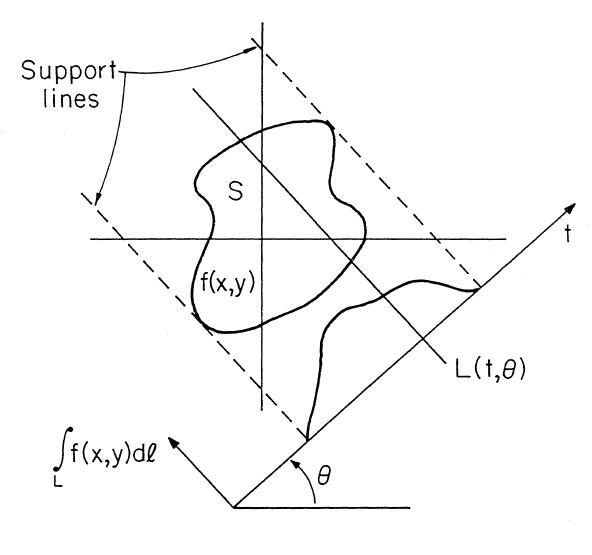
\includegraphics[width=10cm]{images/tomography-application.jpg}
    \caption{Граница носителя функции плотности поглощения определяет две
    опорные прямые к объекту}
    \label{tomography-application}
\end{figure}

По имеющимся измерениям опорной функции можно построить грубое приближение
рассматриваемого тела -- путем обыкновенного пересечения полуплоскостей,
соответствующих опорным прямым. Однако на практике измерения подвержены
ошибкам и известны лишь с некоторой точностью. Так, может оказаться, что
после пересечения построенное тело будет касаться не всех заданных прямых.
Это приводит к тому, что всего одно грубое измерение может заблокировать
воздействие других (более точных) измерений на результат (см. рис.
\ref{inconsistent}).

\begin{figure}[ht]
    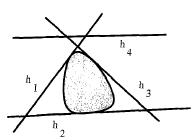
\includegraphics[width=10cm]{images/inconsistent-support-planes.jpg}
    \caption{В случае неточных измерений опорной функции тело нельзя строить
    как пересечение полупространств}
    \label{inconsistent}
\end{figure}

Prince и Willsky рассматривают в своей статье случай, когда измерения опорной
функции получаются по фиксированному набору направлений

\begin{equation}
 u_{i} = (cos \theta_{i}, sin \theta_{i})
\end{equation}

где углы $\theta_{i}$ берутся по всему отрезку $[0, 2 \pi]$ с постоянным шагом:

\begin{equation}
 \theta_{i} = i \cdot \Delta \theta
\end{equation}

где $\Delta \theta = \frac{2 \pi}{M}, i = 0, \ldots, M - 1, M \leq 5$. Более
общий случай, когда направления измерений выбираются произвольным образом,
описывается в статье
\cite[Lele - Kulkarni - Willsky (1992)]{journals/josaa/LeleKW92}.

\subsubsection{Критерий согласованности набора опорных чисел}
\label{sec:history/PrinceW90/criterion}

Ключевым понятием в статье является следующее

\begin{SmartDefinition}
 \label{def:support-vector}
 \textbf{Набором опорных чисел}
 $(h_{0}, h_{1}, \ldots, h_{M - 1})^{T}$выпуклого тела $K$ по заданному набору
 направлений $u_{i}, i = 0, \ldots, M - 1$ называется называется вектор в
 $\mathbb{R}^{M}$, составленный из значений опорной функции по соответствующим
 направлениям: $(h_{K}(u_{0}), h_{K}(u_{1}), \ldots, h_{K}(u_{M - 1}))^{T}$.
\end{SmartDefinition}

Вектор, составленный из набора опорных чисел, является по сути аналогом
непрерывной опорной функции. Если говорить более точно, опорный вектор есть
сеточная функция, соответствующая непрерывной функции $h(\theta)$. Всякая ли
непрерывная функция является опорной функцией некоторого выпуклого тела? Ответ
на этот вопрос дает следующая теорема:

\begin{SmartTheorem}
 \label{thm:support-function-criterion}
 \textbf{Критерий опорной функции}.

 Непрерывная функция $h : \mathbb{R} \to \mathbb{R}_{+}$ является опорной
 функцией некоторого выпуклого тела тогда и только тогда, когда для всех
 $\theta \in \mathbb{R}$ выполнено следующее неравенство:

 \begin{equation}
 h''(\theta) + h(\theta) \geq 0
 \end{equation}
\end{SmartTheorem}


Основным теоретическим результатом статьи, на котором основаны все алгоритмы,
является следующая

\begin{SmartTheorem}
 \label{thm:support-vector-criterion}
 \textbf{Опорная теорема}

 Набор действительных чисел $h \in \mathbb{R}^{M}, M \leq 5$ является набором
 опорных чисел тогда и только тогда, когда

 \begin{equation}
  h^{T} C \leq (0, \ldots, 0)
 \end{equation}

 где $C$ -- $M \times M$ матрица, заданная следующим образом:

 \begin{equation}
  C = 
  \left(
  \begin{array}{ccccccc}
       1 &     -k &      0 & \ldots &      0 &      0 &     -k \\
      -k &      1 &     -k & \ldots &      0 &      0 &      0 \\
       0 &     -k &      1 & \ldots &      0 &      0 &      0 \\
  \vdots & \vdots & \vdots & \ddots & \vdots & \vdots & \vdots \\
       0 &      0 &      0 & \ldots &      1 &     -k &      0 \\
       0 &      0 &      0 & \ldots &     -k &      1 &     -k \\
      -k &      0 &      0 & \ldots &      0 &     -k &      1 \\
  \end{array}
  \right)
 \end{equation}

 где $k = 1 / (2 cos(\frac{2 \pi}{M}))$.
\end{SmartTheorem}

Важно также заметить сходство между условием для непрерывной опорной функции и
условием для дискретного вектора, составленного из набора опорных чисел.
Величина $ - h^{T} C$, компоненты которой должны быть неотрицательными, является
по сути дискретным аналогом величины $h''(\theta) + h(\theta)$. Расширяя эту
аналогию, авторы статьи приводят геометрическую интерпретацию компонент вектора
$ - h^{T} C$ как дискретный радиус кривизны поверхности.

Таким образом, все возможные наборы $h \in \mathbb{R}^{M}$ образуют конус в
$\mathbb{R}^{M}$.

\subsubsection{Опорный конус и его структура}
\label{sec:history/PrinceW90/support-cone}

\begin{SmartDefinition}
 \label{def:support-cone}
 \textbf{Опорным конусом} размерности $M$ называется множество:
 \begin{equation}
 \mathfrak{C} = \{h \in \mathbb{R}^{M} | h^{T} C \leq (0 \ldots 0) \}
 \end{equation}
\end{SmartDefinition}

Дальнейшая часть статьи посвящена, собственно, нахождению такой точки 
$h \in \mathbb{R}^{M}$ в
опорном конусе (т. е. такого набора чисел, который является набором опорных
чисел), который бы соответствовал следующим критериям:

\begin{enumerate}
 \item Расстояние от $h$ до вектора $y \in \mathbb{R}^{M}$, полученного из
измерений, минимально.
 \item Построенное по набору опорных чисел выпуклое тело соответствует
известной априорной информации об объекте.
\end{enumerate}

Под априорной информацией во втором пункте подразумевается, например, известное
положение центра масс вершин полученного многоугольника, или тот факт, что
поверхность тела обладает гладкостью (далее это понятие будет разъяснено).

Прежде всего в статье приводится детальный анализ опорного конуса $\mathfrak{C}$
-- множества, на котором производится минимизация функционала. Поскольку матрица
$C$ циклическая, ее собственные числа можно получить при помощи дискретного
преобразования Фурье ее первой строки (TODO: обосновать). А именно, они равны

\begin{equation}
\lambda_{k} = 1 - \frac{cos(2 \pi (k - 1) / M)}{cos(2 \pi / M)},
k = 1, \ldots, M
\end{equation}

Очевидно, что ровно два собственных значения являются нулевыми:
$\lambda_{2} = \lambda_{M} = 1 - \frac{cos(2 \pi / M)}{cos(2 \pi / M)} = 0$.
Следовательно, матрица $C$ является сингулярной и ее ядро $\mathfrak{N}$ есть
двумерное подпространство, имеющее следующие базисные векторы:

\begin{equation}
n_{1} = (1, cos(\theta_{0}), cos(2 \theta_{0}), \ldots,
cos((M - 1) \theta_{0}))^{T}
\end{equation}

\begin{equation}
n_{2} = (0, sin(\theta_{0}), sin(2 \theta_{0}), \ldots,
sin((M - 1) \theta_{0}))^{T}
\end{equation}

где $\theta_{0} = 2 \pi / M$.

Геометрическим следствием этого факта является то, что конус $\mathfrak{C}$ не
является правильным конусом, поскольку целиком содержит в себе линейное
подпространство размерности 2. Следовательно, опорный конус является декартовым
произведением правильного конуса
$\mathfrak{C}_{p} = \{h \in \mathfrak{C} | h^{T} n_{1} = 0, h^{T} n_{2} = 0\}$
и ядра $\mathfrak{N}$ матрицы $C$. Соответственно, любой вектор, составленный из
набора опорных чисел, является покомпонентной суммой ортогональных векторов
$h_{p} \in \mathfrak{C}_{p}$ и $h_{n} \in \mathfrak{N}$:

\begin{equation}
 h = h_{p} + h_{n}
\end{equation}

Далее в статье показано, что компонента $h_{n}$ есть по сути плоскопараллельный
сдвиг вектора $h$, составленного из набора опорных чисел в пространстве
$\mathbb{R}^{2}$.

\subsubsection{Главная цель набора опорных чисел и ее свойства}
\label{sec:history/PrinceW90/basic-object}

\begin{SmartDefinition}
 \label{def:basic-object}
 Пусть имеется некоторый фиксированный (согласованный) вектор $h$, составленный
 из набора опорных чисел. Тогда существует, вообще говоря, целое семейство
 выпуклых множеств на плоскости $\mathbb{R}^{2}$, для которых вектор $h$
 является вектором опорных чисел. Наибольшее из из этих множеств $S_{B}$ 
 определяется как пересечение полупространств, образованных опорными прямыми:

 \begin{equation}
 S_{B} = \{u \in \mathbb{R}^{2} |
 u^{T} (\omega_{1} \omega_{2} \ldots \omega_{M}) \leq
 (h_{1} h_{2} \ldots h_{M})\}
 \end{equation}

 Данное множество называется \textbf{главной целью} вектора опорных чисел $h$.
\end{SmartDefinition}

В этом месте происходит разделение нашей задачи и той задачи, которую решают
Prince и Willsky в своей статье. А именно, Prince и Willsky полагают, что
главная цель $S_{B}$ является наилучшей оценкой исходного тела. В следующих
разделах будет показано, что в задаче восстановления, которую мы решаем,
ключевую роль играет тот факт, что нам известна структура основных граней камня.

Допустим, что мы прибавляем вектор $h_{n} \in \mathfrak{N}$ из ядра матрицы $C$
к опорному вектору $h$. Что тогда происходит с главной целью? Прежде всего,
можно заметить, что $h_{n}$ можно записать в виде линейной комбинации базисных
векторов пространства $\mathfrak{N}$:

\begin{equation}
h_{n} = v_{1} \left(
  \begin{array}{c}
   n_{1, 1} \\
   n_{1, 2} \\
   \vdots \\
   n_{1, M}
  \end{array}
  \right) + v_{2} \left(
  \begin{array}{c}
   n_{2, 1} \\
   n_{2, 2} \\
   \vdots \\
   n_{2, M} \\
  \end{array}
  \right) = N v
\end{equation}

где $N = \left(
     \begin{array}{cc}
      n_{1, 1} & n_{2, 1} \\
      n_{1, 2} & n_{2, 2} \\
      \vdots & \vdots \\
      n_{1, M} & n_{2, M} \\
     \end{array}
     \right)$ - матрица, столбцы которой составлены из координат базисных
векторов, а
$v = \left(
     \begin{array}{c}
      v_{1} \\
      v_{2} \\
     \end{array}
     \right)$ - вектор-столбец, составленный из коэффициентов линейной
комбинации. Далее, заметим, что главную цель $S_{B}$ опорного вектора
$h = \left(
  \begin{array}{c}
   h_{1} \\
   h_{2} \\
   \vdots \\
   h_{M} \\
  \end{array}
  \right)$ можно записать в следующем виде:

\begin{equation}
S_{B} = \{u \in \mathbb{R}^{2} | N u \leq h\}
\end{equation}

Теперь, прибавляя к неравенству $N u \leq h$ выражение для вектора
$h_{n} = N v$, получаем:
  
\begin{equation}
N (u + v) \leq h + h_{n}
\end{equation}

Таким образом, для каждого $u \in S_{B}$ вектор $u + v$ представляет собой
элемент главной цели вектора $h + h_{n}$. Следовательно, главная цель вектора
$h + h_{n}$ отличается от главной цели вектора $h$ плоскопараллельным сдвигом на
фиксированный вектор $v$.

\subsubsection{Экстремальные вершины и их центр масс}
\label{sec:history/PrinceW90/extreme-points}

Если дан вектор $h = (h_{1}, h_{2}, \ldots, h_{M})$, составленный из набора
опорных чисел некоторого выпуклого тела, то можно явным образом вычислить
координаты вершин главной цели этого вектора (главная цель всегда представляет
собой многоугольник, вершины которого могут быть получены путем
последовательного пересечения соседних опорных прямых):

\begin{equation}
\nu_{i}^{T} = \frac{1}{sin \theta_{0}} (h_{i},  h_{i + 1})
\left(
  \begin{array}{cc}
    sin \theta_{i + 1} & - cos \theta_{i + 1} \\
    - sin \theta_{i} & cos \theta_{i} \\
  \end{array}
\right)
\end{equation}

Вершины главной цели опорного вектора называют \textbf{экстремальными вершинами}
опорного вектора. Примечательно, что центр масс всех экстремальных вершин,
который по сути характеризует абсолютное положение выпуклого тела, представим
в следующем виде:

\begin{equation}
\overline{\nu} = \left(
  \begin{array}{c}
   \overline{\nu}_{x} \\
   \overline{\nu}_{y} \\
  \end{array}
  \right) =
  \frac{1}{M} \sum\limits_{i = 1}^{M} \nu_{i} = \frac{2}{M} N^{T} h
\end{equation}

В данной статье авторы показывают, что данное выражение может быть использовано
в качестве ограничения на опорные векторы -- если положение искомого тела
известно заранее (\textit{a priori}). Заметим, что в частности, когда опорный
вектор $h$ не имеет компоненты в пространстве $\mathfrak{N}$ -- ядре матрицы
$C$, т. е. когда $h \in \mathfrak{C}_{p}$, тогда $N^{T} h = 0$ и, следовательно,
$\overline{\nu} = 0$ -- центр масс главной цели расположен в начале координат.

\subsubsection{Дискретная кривизна и ее свойства}
\label{sec:history/PrinceW90/discrete-curvature}

\begin{figure}[ht]
    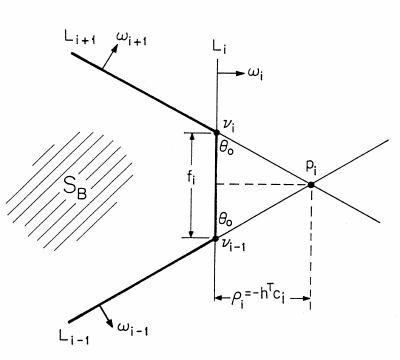
\includegraphics[width=10cm]{images/dicrete-radius-curvature.jpg}
    \caption{Иллюстрация к понятию дискретной кривизны.}
    \label{dicrete-radius-curvature}
\end{figure}

Далее в авторы развивают идею \textbf{дискретного радиуса кривизны} -- величины,
характеризующей гладкость поверхностей главных целей. Представим, что на
рисунке \ref{dicrete-radius-curvature} некоторая материальная точка движется
вдоль $i$-ой стороны многоугольника от экстремальной точки $\nu_{i - 1}$ до
другой экстремальной точки $\nu_{i}$. Тогда во время этого движения вектор
внешней нормали к поверхности меняет угол наклона на величину
$\theta_{0} = \theta_{i} - \theta_{i - 1}$. При этом точка преодолевает
расстояние, равное $f_{i}$. По аналогии с обычным радиусом кривизны,
определяемом как скорость заметания дуги радиусом-вектором поверхности по
отношению к углу наклона радиуса-вектора, авторы определяют дискретный радиус
кривизны как

\begin{equation}
r_{i} = \frac{f_{i}}{\theta_{0}}
\end{equation}

Из геометрических соображений можно показать, что расстояние от точки $p_{i}$
до прямой $L_{i}$ равно $\rho_{i} = -h^{T} c_{i}$, где $c_{i}$ -- $i$-й столбец
матрицы $C$, а из простого тригонометрического соотношения следует, что

\begin{equation}
f_{i} = \frac{2 \rho_{i}}{tg \theta_{0}}
\end{equation}

и, следовательно,

\begin{equation}
\rho_{i} = \frac{1}{2} r_{i} \theta_{0} tg \theta_{0}
\end{equation}

Отсюда следует, что вектор $\rho = - h^{T} C$ состоит из элементов,
пропорциональных дискретным радиусам кривизны $r_{i}$. При этом малые по
величине элементы этого вектора соответствуют "острым" углам, а большие --
"гладким". В дальнейшем авторы статьи используют это соображение в целях
конструирования объекта, гладкость которого известна заранее.

\subsubsection{Общие замечания об алгоритмах восстановления}
\label{sec:history/PrinceW90/algo-common}

Всего Prince и Willsky приводят в статье 3 алгоритма для реконструкции выпуклого
тела по измерениям его опорной функции. При этом предполагается, что измерения
опорной функции получаются как

\begin{equation}
y_{i} = h_{i} + n_{i}, i = 1, \ldots, M
\end{equation}

где $h_{i}$ -- точные значения опорной функции, для которых требуется построить
оценку, а $n_{i}$ -- статистические погрешности, которые представляют собой

\begin{enumerate}
 \item Либо независимые одинаково распределенные гауссовы величины с нулевым
 средним и дисперсией $\sigma^{2}$
 \item Либо независимые случайные величины, равномерно распределенные на отрезке
 $[ - \gamma, \gamma]$.
\end{enumerate}

Вследствие наличия статистических погрешностей измерений нельзя утверждать, что
набор $y = (y_{1}, \ldots, y_{M})$ представляют из себя согласованный набор
опорных чисел. Поэтому первой задачей всех алгоритмов является построение
согласованного набора. Следующей задачей является построение такого
согласованного набора, который бы наилучшим образом соответствовал заранее
известной информации об измеряемом объекте.

\subsubsection{Алгоритм CLOSEST. Алгоритм ближайшего набора}
\label{sec:history/PrinceW90/algo-CLOSEST}

\textbf{Алгоритм ближайшего набора} представляет из себя следующее. В данном
случае предполагается, что статистические погрешности представляют собой
гауссовы величины. В случае, когда отсутствует какая-либо информация об
оцениваемом объекте, следует строить оценку максимального правдоподобия вектора
$h$ по вектору измерений $y$ при условии, что $h \in \mathfrak{C}$:

\begin{equation}
\widehat{h}_{C} = \widehat{h}_{ML} =
\operatornamewithlimits{argmax}_{h: h^{T} C \leq 0}
( - \frac{1}{2} (y - h)^{T} (y - h))
\end{equation}

Очевидно, что данная оценка предоставляет такой вектор $h$ из множества
$\mathfrak{C}$, который является наиболее близким к вектору измерений $y$ в
смысле евклидовой метрики. Если $y \in \mathfrak{C}$, то $\widehat{h}_{C} = y$,
в противном случае оценка $\widehat{h}_{C}$ может быть найдена методами
квадратичного программирования.

\subsubsection{Алгоритм MINI-MAX. Минимаксный алгоритм}
\label{sec:history/PrinceW90/algo-MINI-MAX}


\textbf{Минимаксный алгоритм} предназначен для построения
оценки тела в случае, если заранее известно, что оно представляет из себя тело
с гладкой поверхностью. Для этого строится такая оценка, которая
\textit{максимизирует минимальный радиус кривизны} тела. В такой формулировке
решение всегда будет неограниченным, поскольку многоугольники, вписанные в
концентрические окружности неограниченно возрастающего радиуса, имеют
неограниченный дискретный радиус кривизны. Эту проблему можно решить, если
предположить, что статистические погрешности равномерно распределены на отрезке
$[ - \gamma, \gamma]$. В таком случае каждый реального вектора не может
отстоять от измеренной величины больше чем на $\gamma$. Из этого следует, что
реальный вектор и, следовательно, вектор оценки должен содержаться в гиперкубе

\begin{equation}
\mathfrak{B} = \{h \in \mathbb{R}^{M} |
y - [\gamma, \gamma, \ldots, \gamma]^{T} \leq h \leq
y + [\gamma, \gamma, \ldots, \gamma]^{T}\}
\end{equation}

Таким образом, поскольку величины $\rho_{i} = - h^{T} c_{i}$ пропорциональны
дискретным радиусам кривизны $r_{i}$, авторы статьи определяют минимаксную
оценку как

\begin{equation}
\widehat{h}_{MM} =
\operatornamewithlimits{argmax}_{h \in \mathfrak{C} \cap \mathfrak{B}}
\min_{i = 1, \ldots, M} ( - h^{T} c_{i})
\end{equation}

Решение этой задачи оптимизации может быть получено путем применения методов
линейного программирования. Чтобы показать это, введем новую скалярную величину,
удовлетворяющую следующим неравенствам:

\begin{equation}
\mu \leq - h^{T} c_{i}, i = 1, \ldots, M
\end{equation}

Затем рассмотрим расширенные векторы
$u = \left(
\begin{array}{c}
 h_{1} \\
 h_{2} \\
 \vdots \\
 h_{M} \\
 \mu \\
\end{array}
\right)$ и
$ b = \left(\begin{array}{c}
 0 \\
 0 \\
 \vdots \\
 0 \\
 1 \\
\end{array}
\right)$.

В таких обозначениях нетрудно заметить, что исходная задача может
быть переформулирована как максимизация величины $u^{T} b$ относительно
ограничений $\mu \leq - h^{T} c_{i}, i = 1, \ldots, M$. В такой формулировке и
функционал и неравенства ограничений линейны и, следовательно, задача
максимизации может быть решена методами линейного программирования.

Данный алгоритм наделен одним неудачным свойством: как это часто случается при
применении линейного программирования, решение задачи может быть не
единственным. Очевидно, что, например, прибавление произвольного вектора из ядра
$\mathfrak{N}$ матрицы $C$ не изменяет дискретные кривизны объекта и
следовательно, и функционал, максимизируемый в алгоритме. Следовательно, можно
утверждать, что решением задачи нахождения максиминной оценки является целое
семейство объектов, полученных из исходного методом плоскопараллельных сдвигов в
$\mathbb{R}^{2}$. Минимаксная оценка привязана к величинам, полученным из
измерений только внутри гиперкуба $\mathfrak{B}$, и поэтому при увеличении
$\gamma$ полученная минимаксная все меньше зависит от полученных из эксперимента
данных.

Поэтому минимаксный алгоритм всегда стремится построить многоугольник
наибольшего размера в рамках допустимого гиперкуба, причем этот многоугольник
всегда стремится к окружности. Такие результаты получаются даже если истинное
тело не обладает такими свойствами. Этот недостаток алгоритма послужил для
авторов статьи мотивацией к разработке еще одного алгоритма.

\subsubsection{Алгоритм CLOSE-MIN. Минимаксный алгоритм ближайшего набора}
\label{sec:history/PrinceW90/algo-CLOSE-MIN}

\textbf{Минимаксный алгоритм ближайшего набора} изначально задуман таким
образом, чтобы скомбинировать алгоритм ближайшего набора и минимакный алгоритм.
Сделано это с целью, чтобы получаемая оценка с одной стороны максимально точно
приближала данные, полученные из измерений (как в первом алгоритме), а с другой
-- чтобы учесть заранее известные об объекте данные (как во втором алгоритме).
Идея метода предельно проста: максимизируемый функционал строится как выпуклая
комбинация функционалов двух алгоритмов. С точки зрения статистики алгоритм
представляет собой построение максимальной апостериорной оценки, при этом
слагаемое из алгоритма ближайшего набора играет роль логарифма плотности
измерений (TODO: разобраться в этих понятиях), а слагаемое из минимаксного
алгоритма играет роль логарифма первичной плотности.

Слагаемые берутся с коэффициентами соответственно $\alpha$ и $1 - \alpha$ для
того чтобы дать возможность для настройки алгоритма:

\begin{equation}
\widehat{h}_{CM} =
\operatornamewithlimits{argmax}_{h \in \mathfrak{C} \cap \mathfrak{B}}
(\alpha f_{C}(h) + (1 - \alpha) f_{M}(h))
\end{equation}

где $0 \leq \alpha \leq 1$ и $f_{C}(h)$ и $f_{M}(h)$ представляют из себя
функционалы из первых двух алгоритмов:

\begin{equation}
f_{C}(h) = - \frac{1}{2} (y - h)^{T} (y - h)
\end{equation}

\begin{equation}
f_{M}(h) = \min_{i = 1, \ldots, M} (- h^{T} c_{i})
\end{equation}

Решение данной задачи может быть найдено методами квадратичного
программирования путем расширения вектора $h$, как это было сделано в
минимаксном алгоритме. Заметим, что поскольку $\alpha \neq 0$, условие
принадлежности гиперкубу $\mathfrak{B}$ может быть опущено и решение задачи
является единственным.

\subsubsection{Модификация алгоритмов, учитывающая информацию о абсолютном
положении объекта}
\label{sec:history/PrinceW90/algo-SHIFT-CORRECT}

Предположим, что заранее известно, что центр масс вершин некоторого объекта
расположен в точке $\overline{\nu}$. Тогда данная информация может быть также
заложена в процесс восстановления многоугольника -- восстановленный
многоугольник должен обладать таким же свойством. Данное условие может быть
достигнуто просто путем расширения набора ограничений еще одним линейным
равенством:

\begin{equation}
N^{T} h = \frac{M}{2} \overline{\nu}
\end{equation}

Вследствие линейности данного уравнения внесение его в число ограничений любого
из трех введенных выше алгоритмов не внесет качественных изменений в методы
работы этих алгоритмов (линейное и квадратичное программирование). Эффект от
добавления такого ограничения может быть довольно заметным.

\newpage
\subsection{Методы восстановления многоугольников и их приложения к
задаче распознания цели по данным лазерного радара (по статье Lele, Kulkarni,
Willsky)}
\label{sec:history/LeleKW92}

Дальнейшее развитие рассматриваемая проблема нашла в исследовании авторов Lele,
Kulkarni и Willsky, которое было описано в статье
\cite{journals/josaa/LeleKW92}. Более подробную информацию можно найти в
дипломной работе Lele \cite{thesis/Lele90}.

Данное исследование охватывает совершенно новую область применения --
распознание формы объектов по данным лазерного радара. В ней описано обобщение
первого алгоритма ближайшего набора Prince и Willsky для случая, когда
направления, по которым производится измерение опорной функции, распределены
произвольным образом. Также в ней вводится 2 новых алгоритма, которые позволяют
строить тело на основе априорной информации о количестве его сторон и
либо направлениях нормалей этих сторон, либо об относительных углах между этими
направлениями.

\subsubsection{Алгоритм NUA. Восстановление многоугольника со сторонами по
углам измерения}
\label{sec:history/LeleKW92/algo-NUA}

Данный алгоритм является обобщением алгоритма ближайшего набора из статьи Prince
и Willsky, в котором тело строится по конечному набору величин
$y_{1}, y_{2}, \ldots, y_{M}$,  которые представляют собой измеренные с
погрешностями значениями опорной функции по направлениям вдоль известных углов
$\theta_{1} < \theta_{2} < \ldots < \theta_{M}$, которые называются
\textbf{углами измерения}. Отличие от упомянутого алгоритма состоит в том, что
критерий матрица в неравенстве из критерия согласованности записывается
несколько иным образом.

Тройка опорных чисел $h_{i - 1}, h_{i}, h_{i + 1}$ по углам $\theta_{i - 1},
\theta_{i}, \theta_{i + 1}$ является согласованной тогда и только тогда, когда
выполнено следующее неравенство:

\begin{equation}
h_{i - 1} sin(\theta_{i + 1} - \theta_{i}) -
h_{i} sin(\theta_{i + 1} - \theta_{i - 1}) +
h_{i + 1} sin(\theta_{i} - \theta_{i - 1}) \geq 0
\end{equation}

Опорная теорема теперь записывается следующим образом:

\begin{SmartTheorem}
 \label{thm:ext-support-theorem-2d}
 \textbf{Обобщенная двумерная опорная теорема}.
 Набор действительных чисел
 $h = (h_{1}, h_{2}, \ldots, h_{M}) \in \mathbb{R}^{M}$
 является набором опорных чисел по направлениям вдоль углов
 $\theta_{1} < \theta_{2} < \ldots < \theta_{M}$ тогда и только тогда, когда
 выполнено следующее матричное неравенство:

 \begin{equation}
 C h \geq 0
 \end{equation}

 где матрица $C$ представляет собой следующее:

 \begin{equation}
  \left(
  \begin{array}{ccccccc}

   \scriptstyle     -sin(\theta_{2} - \theta_{M}) &
   \scriptstyle     sin(\theta_{1} - \theta_{M}) &
   \scriptstyle     0 &
   \scriptstyle     \ldots &
   \scriptstyle     0 &
   \scriptstyle     0 &
   \scriptstyle     sin(\theta_{2} - \theta_{1}) \\

   \scriptstyle      sin(\theta_{3} - \theta_{2}) &
   \scriptstyle      -sin(\theta_{3} - \theta_{1}) &
   \scriptstyle      sin(\theta_{2} - \theta_{1}) &
   \scriptstyle      \ldots &
   \scriptstyle      0 &
   \scriptstyle      0 &
   \scriptstyle      0 \\

   \scriptstyle      0 &
   \scriptstyle      sin(\theta_{4} - \theta_{3}) &
   \scriptstyle      -sin(\theta_{4} - \theta_{2}) &
   \scriptstyle      \ldots &
   \scriptstyle      0 &
   \scriptstyle      0 &
   \scriptstyle      0 \\

   \scriptstyle      \vdots &
   \scriptstyle      \vdots &
   \scriptstyle      \vdots &
   \scriptstyle      \ddots &
   \scriptstyle      \vdots &
   \scriptstyle      \vdots &
   \scriptstyle      \vdots \\

   \scriptstyle      0 &
   \scriptstyle      0 &
   \scriptstyle      0 &
   \scriptstyle      \ldots &
   \scriptstyle      -sin(\theta_{M - 1} - \theta_{M - 3}) &
   \scriptstyle      sin(\theta_{M - 2} - \theta_{M - 3}) &
   \scriptstyle      0 \\

   \scriptstyle      0 &
   \scriptstyle      0 &
   \scriptstyle      0 &
   \scriptstyle      \ldots &
   \scriptstyle      sin(\theta_{M} - \theta_{M - 1}) &
   \scriptstyle      -sin(\theta_{M} - \theta_{M - 2}) &
   \scriptstyle      sin(\theta_{M - 1} - \theta_{M - 2}) \\

   \scriptstyle      sin(\theta_{M} - \theta_{M - 1}) &
   \scriptstyle      0 &
   \scriptstyle      0 &
   \scriptstyle      \ldots &
   \scriptstyle      0 &
   \scriptstyle      sin(\theta_{1} - \theta_{M}) &
   \scriptstyle      -sin(\theta_{1} - \theta_{M - 1}) \\
  \end{array}
  \right)
 \end{equation}
\end{SmartTheorem}

Данный алгоритм авторы называют NUA (от nonuniform angles).

\subsubsection{Алгоритм BNGON. Наилучший N-угольник по M измерениям с заданными
углами восстановления}
\label{sec:history/LeleKW92/algo-BNGON}

Данный алгоритм был разработан для случая, когда известна следующая априорная 
информация об объекте: точное количество сторон многоугольника и углы наклона 
нормалей к этим сторонам (эти углы далее будут называться \textbf{углами
восстановления}). Такая информация позволяет получать более качественную оценку
многоугольника.

Обозначим углы измерений через $\{\theta_{1}, \theta_{2}, \ldots,
\theta_{M}\}$, величины приближенно измеренных опорных чисел через $\{y_{1},
y_{2}, \ldots, y_{M}\}$, а известные углы восстановления через $\{\phi_{1},
\phi_{2}, \ldots, \phi_{N}\}$. По этим данным требуется построить N-угольник,
определяемый  согласованным набором опорных чисел $\{h_{\phi}(\phi_{1}),
h_{\phi}(\phi_{2}), \ldots, h_{\phi}(\phi_{N})\}$ по заданным углам
восстановления, который доставляет минимум для следующего функционала:

\begin{equation}
J[h_{\phi}(\phi_{1}), h_{\phi}(\phi_{2}), \ldots, h_{\phi}(\phi_{N})] =
\sum \limits_{i = 1}^{M}[h_{\phi}(\theta_{i}) - y_{i}]^{2}
\end{equation}

Как известно, опорная функция многоугольника представляет собой
кусочно-синусоидальную функцию. Поэтому значения $h_{\phi}(\theta_{i})$ всегда 
можно вычислить следующим образом:

\begin{enumerate}
 \item Найти соседние углы восстановления $\phi_{L_{i}}$ и $\phi_{R_{i}}$
такие, что $\phi_{L_{i}} < \theta_{i} < \phi_{R_{i}}$ и на отрезке
$[\phi_{L_{i}}, \phi_{R_{i}}]$ нет других углов восстановления.
 \item Вычислить $h_{\phi}(\theta_{i})$ по следующей формуле:
\end{enumerate}

\begin{equation}
h_{\phi}(\theta_{i}) =
\frac{sin(\phi_{R_{i}} - \theta_{i})}{sin(\phi_{R_{i}} - \phi_{L_{i}})}
h_{L_{i}} +
\frac{sin(\theta_{i} - \phi_{L_{i}})}{sin(\phi_{R_{i}} - \phi_{L_{i})}}
h_{R_{i}}
\end{equation}

Используя это соотношение, задачу минимизации можно переформулировать следующим
образом:

\begin{equation}
\widehat{h}_{\phi} = \left(
\begin{array}{c}
 \widehat{h}_{\phi}(\phi_{1}) \\
 \widehat{h}_{\phi}(\phi_{2}) \\
 \vdots \\
 \widehat{h}_{\phi}(\phi_{N}) \\
\end{array}
\right) = \operatornamewithlimits{argmin}_{C h_{\phi} \geq 0} (A h_{\phi} -
y)^{T} (A h_{\phi} - y)
\end{equation}

где $A$ есть $M \times N$ матрица, строками которой являются коэффициенты
линейных комбинаций элементов вектора $h_{\phi} = [h_{\phi}(\phi_{1})c,
h_{\phi}(\phi_{2}), \ldots, {\phi}(\phi_{N})]^{T}$, через которые
выражаются соответствующие опорные числа $h_{\phi}(\theta_{1}),
h_{\phi}(\theta_{2}), \ldots, h_{\phi}(\theta_{M})$ по углам измерений.

Поскольку рассматриваемый функционал является квадратичным, а ограничения на
условия минимизации являются линейными, искомый минимум может быть найден с
помощью стандартных методов квадратичного программирования.

В статье авторы называют этот алгоритм BNGON (best N-gon).

\subsubsection{Алгоритм BNGONROT. Наилучший N-угольник по M измерениям с
заданными относительными углами}
\label{sec:history/LeleKW92/algo-BNGONROT}

Данный алгоритм предназначен для случая, когда о теле доступна несколько
меньшая информация, а именно известны относительные углы между нормалями, но
абсолютные значения этих углов неизвестны.

Пусть как и раньше $\{\theta_{1}, \theta_{2}, \ldots,
\theta_{M}\}$ суть углы измерений, а величины приближенно измеренных опорных
чисел суть $\{y_{1}, y_{2}, \ldots, y_{M}\}$. Отличие от предыдущего алгоритма 
состоит в том, что углами восстановления являются $\{\phi_{1} + \alpha,
\phi_{2} + \alpha, \ldots, \phi_{N} + \alpha\}$, где $\{\phi_{1}, \phi_{2},
\ldots, \phi_{N}\}$ известны, а $\alpha \in [0, 2 \pi]$ служит неизвестным
смещением углов восстановления.

Минимизируемым функционалом в данном случае является

\begin{equation}
J[\alpha, h_{\phi}(\phi_{1} + \alpha), h_{\phi}(\phi_{2} + \alpha), \ldots,
h_{\phi}(\phi_{N} + \alpha)] =
\sum \limits_{i = 1}^{M}[h_{\phi}(\theta_{i}) - y_{i}]^{2}
\end{equation}

причем величины $h_{\phi}(\theta_{i})$ вычисляются по похожей формуле

\begin{equation}
h_{\phi}(\theta_{i}) =
\frac{sin(\phi_{R_{i}} + \alpha - \theta_{i})}{sin(\phi_{R_{i}} - \phi_{L_{i}})}
h_{L_{i}} +
\frac{sin(\theta_{i} - \phi_{L_{i}} - \alpha)}{sin(\phi_{R_{i}} - \phi_{L_{i})}}
h_{R_{i}}
\end{equation}

Однако данный функционал не является квадратичным вследствие того, что
неизвестная $\alpha$ входит в выражение через аргументы тригонометрических
функций. Тем не менее, авторы приводят основанный на квадратичном 
программировании алгоритм, который позволяет решить эту задачу.

Обозначим через $J_{h_{\phi}}(\alpha)$ минимум функционала по значениям опорных 
чисел при фиксированном значении смещения $\alpha$.

\begin{equation}
J_{h_{\phi}}(\alpha) = \min_{{h_{\phi}(\phi_{i} + \alpha)}} J[\alpha,
h_{\phi}(\phi_{1} + \alpha), h_{\phi}(\phi_{2} + \alpha), \ldots,
h_{\phi}(\phi_{N} + \alpha)]
\end{equation}

Самым простым решением данной задачи является решение методом грубой
силы: перебор некоторого большого набора величин смещений $\alpha$, взятых с
определенным шагом. Такой подход является, без сомнения, довольно трудоемким.
Поэтому авторы разработали более эффективный градиентный алгоритм. Сущность
задачи внесла два важных отличия в этот алгоритм по сравнению с обычным
алгоритмом градиентного спуска. Во-первых, заметим что

\begin{equation}
J_{h_{\phi}}(\alpha) = J[\alpha,
h_{\phi}^{*}(\phi_{1} + \alpha), h_{\phi}^{*}(\phi_{2} + \alpha), \ldots,
h_{\phi}^{*}(\phi_{N} + \alpha)]
\end{equation}

где величины $h_{\phi}^{*}(\phi_{i} + \alpha)$ доставляют минимум для
функционала $J_{h_{\phi}}(\alpha)$. Поэтому

\begin{equation}
\frac{d J_{h_{\phi}}(\alpha)}{d \alpha} = \frac{\partial J}{\partial \alpha} +
\sum \limits_{i = 1}^{N} \frac{\partial J}{\partial h_{\phi}(\phi_{i} + \alpha)}
\frac{\partial h_{\phi}^{*}(\phi_{i} + \alpha) }{\partial \alpha}
\end{equation}

Здесь вычисление величины
$\frac{\partial h_{\phi}^{*}(\phi_{i} + \alpha)}{\partial \alpha}$ представляет
большую трудность, поскольку вычисление каждого значения
$h_{\phi}^{*}(\phi_{i} + \alpha)$ требует решения задачи квадратичного
программирования. Поэтому авторы приняли решение использовать в градиентном
методе не полную, а лишь частную производную:

\begin{equation}
\frac{\partial J}{\partial \alpha} [\alpha,
h_{\phi}^{*}(\phi_{1} + \alpha), h_{\phi}^{*}(\phi_{2} + \alpha), \ldots,
h_{\phi}^{*}(\phi_{N} + \alpha)] =
2 \sum \limits_{i = 1}^{M}  \frac{\partial h_{\phi}(\theta_{i}) }{\partial
\alpha} [h_{\phi}^{*}(\theta_{i}) - y(\theta_{i})]
\end{equation}

где используя известное выражение для опорных чисел в углах измерения через
опорные числа в углах восстановления можно получить:

\begin{equation}
\frac{\partial h_{\phi}(\theta_{i})}{\partial \alpha} =
\frac{cos(\phi_{R_{i}} + \alpha - \theta_{i})}{sin(\phi_{R_{i}} - \phi_{L_{i}})}
h_{L_{i}} +
\frac{cos(\theta_{i} - \phi_{L_{i}} - \alpha)}{sin(\phi_{R_{i}} - \phi_{L_{i})}}
h_{R_{i}}
\end{equation}

Вторым важным отличием представленного алгоритма является то, что функция
$J_{h_{\phi}}(\alpha)$ является, вообще говоря, сильно невыпуклой функцией от
$\alpha$ (авторы отсылают на \cite{thesis/Lele90}, где этот вопрос рассмотрен
более детально). Данный факт приводит к тому, что для решения задачи нужно
найти все возможные локальные минимумы функционала. Авторы предлагают делать это
следующим образом.

\begin{enumerate}
 \item Положить $\alpha = 0$.
 \item Вычислить $\frac{\partial J}{\partial \alpha}$.
 \item Если $\frac{\partial J}{\partial \alpha} > 0$, сделать шаг градиентного 
подъема, в противном случае -- шаг градиентного спуска.
 \item Если изменение величины функционала не превышает заданный порог
$\epsilon$, то сообщить о найденном локальном минимуме и перейти к шагу 7.
 \item Если знак функционала не поменялся, вернуться к шагу 2
 \item Если знак функционала поменялся, то методом деления пополам найти точку 
изменения знака и сообщить, что в ней есть локальный минимум.
 \item Если $\alpha < 2 \pi$, увеличить $\alpha := \alpha + \delta \alpha$ и
вернуться к шагу 2 для того, чтобы найти еще один локальный минимум. В противном
случае завершить алгоритм.
\end{enumerate}

Затем нужно найти оптимальный минимум среди сообщенных данным алгоритмом.

В статье авторы называют этот алгоритм BNGONROT (best N-gon with rotations).

\subsubsection{Сравнительный анализ погрешностей трех алгоритмов}
\label{sec:history/LeleKW92/analysis}

Авторы проводили довольно аккуратный и детальный анализ приведенных алгоритмов:

\begin{enumerate}
 \item Анализ алгоритмов на синтетических объектах (равнобедренный треугольник).
 \item Анализ алгоритмов для обработки данных, полученных в лабораторных
условиях.
 \item Анализ алгоритмов в "полевых" условиях, т. е. на реальных лазерных
радарах.
 \item Статистическое обоснование смещенности получаемых оценок (по критерию
Крамера-Рао).
 \item Статистический анализ погрешностей алгоритмов на данных, симулированных
методом Монте-Карло.
\end{enumerate}

При этом важным является тот факт, что авторы везде брали очень большие
величины погрешностей (например, $\sigma = 0.25$ для объектов со сторонами 
длины $0.5$), что видимо отражает специфику рассматриваемых ими данных.

Одним из результатов этого анализа является то, что алгоритмы BNGON и BNGONROT
предоставляют погрешности меньшие, чем погрешность алгоритма NUA примерно в 10
раз. Разница же между погрешностями BNGON и BNGONROT гораздо меньше.

\subsubsection{Приложение алгоритмов к распознаванию объектов с помощью
лазерного радара}
\label{sec:history/LeleKW92/applications}

Также авторы описывают методы извлечения информации об опорных прямых к
объекту, которые они использовали в экспериментах. Было также проведено
исследование, которое показало, что алгоритмы успешно помогают обрабатывать
данные, возникающие в компьютерной томографии.

\newpage
\subsection{Локальные тесты для проверки согласованности измерений опорной
функции (по статье Karl, Kulkarni, Verghese, Willsky)}
\label{sec:history/KarlKVW96}

Основным предметом исследования статьи является поиск набора условий,
являющийся критерием согласованности набора измерений опорной функции 
произвольного выпуклого тела в $\mathbb{R}^{N}$. Новизна статьи состоит в
том, что задача рассматривается для случая произвольной размерности. При этом
авторы строят набор условий, исходя из их практической применимости в реальных
алгоритмах восстановления.

\subsubsection{Критерий опорной функции в $\mathbb{R}^{n}$}
\label{sec:history/KarlKVW96/support-function-criterion}

Довольно естественным вопросом, который возникает пр рассмотрении опорных
функций является следующий: какие функции могут быть опорными для некоторого
тела? Ответ на этот вопрос дает следующая классическая теорема:

\begin{SmartTheorem}
 \label{thm:support-function-criterio-R2}
 \textbf{Критерий опорной функции}.
 Функция $H(v): \mathbb{R}^{2} \to \mathbb{R}$ является опорной функцией
 некоторого выпуклого тела тогда и только когда она определена на всем
 $\mathbb{R}^{n}$ и удовлетворяет следующим свойствам:
 \begin{enumerate}
  \item $H(0) = 0$.
  \item $H(\alpha v) = \alpha H(v)$ для всех $\alpha > 0$.
  \item $H(v + w) \leq H(v) + H(w)$ для всех $v, w \in \mathbb{R}^{n}$
 \end{enumerate}
\end{SmartTheorem}

Впервые доказательство данной теоремы было представлено Минковским для случая
трехмерной размерности, а позже в работе \cite{journals/mz/Rademacher22}
Радемахером было произведено обобщение на случай произвольной размерности.
Неудобство этой теоремы с точки зрения приложений состоит в том, что условие,
которое ей формулируется, является \textit{глобальным}, в том смысле, что оно
должно быть проверяемо для каждой пары векторов $v$ и $w$ в $\mathbb{R}^{n}$.

Потому Радемахер показал, что 3-е условие теоремы может быть заменено другим.
А именно, было показано, что при условиях 1 и 2 теоремы
\ref{thm:support-function-criterio-R2} условие 3 эквивалентно следующему:

\begin{SmartTheorem}
 \label{thm:support-function-criterio-R2-det}
 \textbf{Детерминантный критерий опорной функции}.
 Функция $H(v): \mathbb{R}^{2} \to \mathbb{R}$ является опорной функцией
 некоторого выпуклого тела тогда и только когда выполнены условия 1 и 2 из
 теоремы \ref{thm:support-function-criterio-R2} а также следующее условие:

\begin{equation}
 \left|\begin{array}{cc}
  h(u_{1}) & u_{1}^{T} \\
  h(u_{2}) & u_{2}^{T} \\
  h(u_{3}) & u_{3}^{T} \\
 \end{array}\right|
  \left|\begin{array}{cc}
  1 & u_{1}^{T} \\
  1 & u_{2}^{T} \\
  1 & u_{3}^{T} \\
 \end{array}\right|
 \geq 0
\end{equation}
для всевозможных троек единичных векторов $u_{1}, u_{2}, u_{3}$.
\end{SmartTheorem}

Теперь в отличие данной теоремы от критерия опорной функции (см. теорему
\ref{thm:support-function-criterion}) состоит в том, что она не требует
дифференцируемости, но формулирует условие прямо в терминах
\textit{экспериментально измеряемых величин} $h(u)$.

Предположим, что все числа $u_{1}$, $u_{2}$, $u_{3}$ различны и что $u_{3}$
лежит в либо в положительной, либо в отрицательной части конуса для точек
$\{u_{1}, u_{2}\}$ (этого условия можно достичь просто путем переименования
переменных).

Также авторы статьи показывают, что последнее условие теоремы
\ref{thm:support-function-criterio-R2-det} эквивалентно следующему:

\begin{equation}
 \beta \left( u_{3}^{T}
 \left[
 \begin{array}{c}
 u_{1}^{T} \\
 u_{2}^{T} \\
 \end{array}
 \right]^{-1}
 \left[
 \begin{array}{c}
 h(u_{1}) \\
 h(u_{2}) \\
 \end{array}
 \right] - h(u_{3}) \right) \geq 0
\end{equation}

где скалярная функция $\beta = \beta(u_{1}, u_{2}, u_{3})$ зависит только от
набора чисел $u_{i}$. При этом если $u_{3}$ лежит в положительном конусе для
$\{u_{1}, u_{2}\}$, то $\beta(u_{1}, u_{2}, u_{3}) \geq 0$, а если в
отрицательном -- то $\beta(u_{1}, u_{2}, u_{3}) < 0$.

Однако данные условия все еще являются глобальными, поскольку требуют проверки
по всем возможным тройкам единичных векторов $(u_{1}, u_{2}, u_{3})$.

Результат Радемахера был обобщен на случай произвольной размерности:

\begin{SmartTheorem}
 \label{thm:support-function-criterio-ext}
 \textbf{Обобщенный критерий опорной функции}.
 Функция $H(v): \mathbb{R}^{n} \to \mathbb{R}$ является опорной функцией
 некоторого выпуклого тела в $\mathbb{R}^{n}$ тогда и только когда она
 определена на всем $\mathbb{R}^{n}$ и удовлетворяет следующим свойствам:
 \begin{enumerate}
  \item $H(0) = 0$.
  \item $H(\alpha v) = \alpha H(v)$ для всех $\alpha > 0$.
  \item Следующее детерминантное неравенство выполняется для каждого набора из
  $n + 1$ единичных векторов $u_{i}$, в котором один из векторов лежит в полном
  положительном конусе основных:
\begin{equation}
\label{thm:support-function-criterio-ext:condition}
 \left|\begin{array}{cc}
  h(u_{1}) & u_{1}^{T} \\
  h(u_{2}) & u_{2}^{T} \\
  \vdots & \vdots \\
  h(u_{n + 1}) & u_{n + 1}^{T} \\
 \end{array}\right|
  \left|\begin{array}{cc}
  1 & u_{1}^{T} \\
  1 & u_{2}^{T} \\
  \vdots & \vdots \\
  1 & u_{n + 1}^{T} \\
 \end{array}\right|
 \geq 0
\end{equation}

 \end{enumerate}
\end{SmartTheorem}

Точно так же, как и в плоском случае, можно показать, что последнее неравенство
эквивалентно следующему:

\begin{equation}
\label{thm:support-function-criterio-ext:condition2}
 u_{n + 1}^{T}
 \left[
 \begin{array}{c}
 u_{1}^{T} \\
 u_{2}^{T} \\
 \vdots \\
 u_{n}^{T} \\
 \end{array}
 \right]^{-1}
 \left[
 \begin{array}{c}
 h(u_{1}) \\
 h(u_{2}) \\
 \vdots \\
 h(u_{n}) \\
 \end{array}
 \right] - h(u_{n + 1}) \geq 0
\end{equation}

\subsubsection{Критерий набора опорных чисел в $\mathbb{R}^{n}$}
\label{sec:history/KarlKVW96/support-vector-criterion}

Как упоминалось ранее, измерения опорной функции, которые получаются из
экспериментальных данных, содержат погрешности, которые приводят к тому, что
набор перестает быть согласованным. Чтобы восстановить согласованность набора,
нужно ввести ряд условий, который будет задавать множество всех наборов опорных
чисел.

\begin{SmartTheorem}
 \label{thm:discrete-consistency}
 \textbf{Критерий набора опорных чисел в $\mathbb{R}^{n}$}.
 Набор действительных чисел $h = (h_{1}, h_{2}, \ldots, h_{N})$ по
 направлениям $u_{1}, u_{2}, \ldots, u_{N}$ является набором  опорных чисел
 некоторого выпуклого тела в $\mathbb{R}^{n}$ тогда и только тогда, когда
 каждый поднабор $h_{(i_{1}, i_{2}, \ldots i_{n + 1})} = \{h_{i_{1}}, h_{i_{2}},
 \ldots, h_{i_{n + 1}}\}$ из $n + 1$ чисел удовлетворяет следующему условию:

 Для каждого числа $h_{i_{j}}$ из $(n + 1)$-поднабора гиперплоскость,
 соответствующая числу, имеет непустое пересечение с пересечением всех $n + 1$
 соответствующих полупространств:

 \begin{equation}
 \label{thm:discrete-consistency:condition}
  \pi(h_{i_{j}}, u_{i_{j}}) \cap \bigcap \limits_{k = 1}^{n + 1} R(h_{i_{k}}, 
  u_{i_{k}}) \neq \varnothing \;\;\; \forall j = 1, 2, \ldots, n + 1
 \end{equation}

 где через
 $\pi(h, u) = \{x \in \mathbb{R}^{n} \; | \; (x, u) = h\}$
 обозначается  гиперплоскость, а через
 $R(h, u) = \{x \in \mathbb{R}^{n} \; | \; (x, u) \leq h\}$
 -- полупространство, соответствующие опорному числу $h$ по направлению $u$.
\end{SmartTheorem}

Фактически последнее условие является обобщением геометрической интерпретации,
изображенной на рис. \ref{dicrete-radius-curvature}. Недостаток данной теоремы
с точки зрения приложений состоит в том, что условие должно быть проверено для
всех возможных $(n + 1)$-поднаборов, т. е. оно не является \textit{локальным}.
Вследствие этого авторы посвятили оставшуюся часть статьи сокращению числа
условий, которые должны быть проверены.

\subsubsection{Локальный критерий набора опорных чисел в $\mathbb{R}^{n}$}
\label{sec:history/KarlKVW96/support-vector-criterion-local}

Главным результатом статьи является сокращение числа условий до того, что 
критерий становится локальным. Во-первых, проводится классификация $(n + 
1)$-поднаборов:

\begin{SmartDefinition}
 \label{def:tuples-classifiction}
 Пусть имеется набор $(u_{1}, u_{2}, \ldots, u_{n + 1})$ из $n + 1$ векторов в
 $\mathbb{R}^{n}$. Тогда он называется
 \begin{enumerate}
  \item \textbf{конусно-положительным}, если один из векторов $u_{i}$
  положительной конусной оболочке остальных.
  \item \textbf{конусно-отрицательным}, если один из векторов $u_{i}$
  отрицательной конусной оболочке остальных.
  \item \textbf{конусно-нейтральным} -- в противном случае.
 \end{enumerate}
\end{SmartDefinition}

Последний класс наборов -- конусно-нейтральный -- не представляет интереса для
исследования, поскольку в нем условие \ref{thm:discrete-consistency:condition}
из теоремы \ref{thm:discrete-consistency} выполняется автоматически. Более
того, при условии что
$\bigcap \limits_{i = 1}^{N} R(h_{i}, u_{i}) \neq \varnothing$,
т. е. пересечение всех соответствующих опорным числам полупространств непусто,
условие \ref{thm:discrete-consistency:condition} выполняется автоматически и 
для конусно-отрицательных наборов.

Далее, если конусно-положительный набор является невырожденным, т. е.
соответствующая конусная оболочка является \textit{полной}, то условие
\ref{thm:discrete-consistency:condition} из теоремы
\ref{thm:discrete-consistency} эквивалентно детерминантному условию
\ref{thm:support-function-criterio-ext:condition} из теоремы
\ref{thm:support-function-criterio-ext}, или эквивалентному ему матричному
условию \ref{thm:support-function-criterio-ext:condition2}.

Данные соображения используются для введения следующего критерия:

\begin{SmartTheorem}
 \label{thm:positive-cone-consistency}
 \textbf{Конусно-положительный критерий набора опорных чисел в $\mathbb{R}^{n}$}
 Пусть имеется набор действительных чисел $h = (h_{1}, h_{2}, \ldots, h_{N})$ по
 направлениям $u_{1}, u_{2}, \ldots, u_{N}$. Пусть выполнены следующие 
 условия:
 \begin{enumerate}
  \item Пересечение всех соответствующих полупространств непусто:
  \begin{equation}
   \bigcap \limits_{i = 1}^{N} R(h_{i}, u_{i}) \neq \varnothing
  \end{equation}
  \item Для каждого конусно-положительного $(n + 1)$-поднабора конусная оболочка
  является полной.
 \end{enumerate}

 Тогда данный набор является набором опорных чисел некоторого выпуклого тела в 
 $\mathbb{R}^{n}$ тогда и только тогда, когда условие 
 \ref{thm:support-function-criterio-ext:condition} из теоремы
 \ref{thm:support-function-criterio-ext} выполняется для каждого 
 конусно-положительного $(n + 1)$-поднабора чисел.
\end{SmartTheorem}

Далее авторы статьи с помощью идеи, которую они называют \textbf{слиянием 
согласованности}, проводят сведение глобального критерия согласованности к 
локальному:

\begin{SmartLemma}
 \label{lem:consistency-merging}
 \textbf{Слияние согласованности}.
 Пусть имеется множество из $(n + 2)$ опорных чисел $h_{i}$ по направлениям 
 $u_{i}$ в $\mathbb{R}^{n}$ и пусть выполнены следующие условия:
 
 \begin{enumerate}
  \item $u_{n + 1} \in cone^{+}\{u_{1}, \ldots, u_{n - 1}, u_{n + 2}\}$
  \item $u_{n + 2} \in cone^{+}\{u_{2}, \ldots, u_{n}, u_{n + 1}\}$
  \item $\{u_{n + 1}, u_{n + 2}\} \in cone^{+}\{u_{1}, \ldots, u_{n - 1},
u_{n}\}$
  \item Все три этих конуса являются полными.
 \end{enumerate}

 Тогда если наборы опорных чисел 
 $\{h_{1}, \ldots, h_{n - 1}, h_{n + 1}, h_{n + 2}\}$ и
 $\{h_{2}, \ldots, h_{n}, h_{n + 1}, h_{n + 2}\}$ согласованы, то и наборы
 $\{h_{1}, \ldots, h_{n}, h_{n + 1}\}$ и
 $\{h_{1}, \ldots, h_{n}, h_{n + 2}\}$ также являются согласованными.
\end{SmartLemma}

Для того, чтобы конкретизировать понятие \textit{локальности}, авторы статьи
вводят следующее определение:

\begin{SmartDefinition}
 \label{def:local-family}
 \textbf{Локальное семейство}.
 Пусть имеется набор $\mathit{S}$ из $m$ различных единичных векторов в
 $\mathbb{R}^{n}$. Пусть $u_{k}$ - один из этих векторов. Тогда
 \textbf{локальным семейством}, соответствующим вектору $u_{k}$, называется 
 множество всех различных $(n + 1)$-поднаборов $u_{i_{1}, \ldots, 
 i_{n}} = \{u_{k}, u_{i_{1}}, u_{i_{2}}, \ldots, u_{i_{n}}\}$ векторов из 
 $\mathit{S}$ таких,
 что:
 \begin{enumerate}
  \item $u_{k}$ является элементом этого $(n + 1)$-поднабора (это видно и по 
  определению этого поднабора как $u_{i_{1}, \ldots, 
 i_{n}} = \{u_{k}, u_{i_{1}}, u_{i_{2}}, \ldots, u_{i_{n}}\}$).
  \item Полная положительная конусная оболочка векторов $\{u_{i_{1}}, 
  u_{i_{2}}, \ldots, u_{i_{n}}\}$ содержит векторы $u_{k}, u_{i_{1}}, u_{i_{2}}, 
  \ldots, u_{i_{n}}$ и не содержит никаких других векторов из $\mathit{S}$.
 \end{enumerate}
\end{SmartDefinition}

Основным результатом статьи является следующая теорема, которая представляет
собой локальный критерий согласованности набора опорных чисел:

\begin{SmartTheorem}
 \label{thm:local-global-consistency-equivalence}
 \textbf{Локальный критерий набора опорных чисел в $\mathbb{R}^{n}$}.
 Пусть имеется набор действительных чисел $h = (h_{1}, h_{2}, \ldots, h_{N})$ по
 направлениям $u_{1}, u_{2}, \ldots, u_{N}$. Пусть выполнены следующие 
 условия:
 \begin{enumerate}
  \item Пересечение всех соответствующих полупространств непусто:
  \begin{equation}
   \bigcap \limits_{i = 1}^{N} R(h_{i}, u_{i}) \neq \varnothing
  \end{equation}
  \item Для каждого конусно-положительного $(n + 1)$-поднабора конусная оболочка
  является полной.
 \end{enumerate}

 Тогда данный набор является набором опорных чисел некоторого выпуклого тела в 
 $\mathbb{R}^{n}$ тогда и только тогда, когда условие 
 \ref{thm:support-function-criterio-ext:condition} из теоремы
 \ref{thm:support-function-criterio-ext} выполняется для каждого направляющего
 вектора $u_{k}$ опорные числа $\{h_{k}, h_{i_{1}}, \ldots, h_{i_{n}}\}$, 
 соответствующие направлениям $\{u_{k}, u_{i_{1}}, \ldots, h_{u_{n}}\}$ из 
 локального семейства $u_{k}$.
\end{SmartTheorem}

Таким образом, результаты Prince и Willsky из
статьи \cite{journals/pami/PrinceW90}, который рассмотрен в разделе
\ref{sec:history/PrinceW90}, можно расширить на случай задач произвольной
размерности. Пусть $t = |\bigcup \limits_{i = 1}^{N} LF_{i}|$ - число элементов
локальных семейств всех направлений (через $LF_{i}$ обозначено $i$-е локальное 
семейство). Тогда можно сформулировать все те задачи минимизации, которые
рассматривали Prince и Willsky, с тем лишь отличием, что вместо условия
$Ch \leq 0$ должно быть использовано условие

\begin{equation}
 Q h \geq 0
\end{equation}

где $Q$ -- $t \times m$ матрица, составленная из коэффициентов линейных
комбинаций условий согласованности для каждого набора из каждого локального
семейства. При этом каждая строка этой матрицы содержит не более $n + 1$
ненулевых коэффициентов.

\newpage
\subsection{Применение методов построения оценок опорных функций к задачам
магнитно-резонансной визуализации (по статьям Gregor и Rannou)}

Алгоритмы оптимизации, предложенные Karl, Kulkarni, Verghese, Willsky в статье
\cite{journals/jmiv/KarlKVW96}, как кажется, до сих пор еще не нашли применения
в крупных производственных системах. Единственной известной на
сегодняшний день попыткой является применение данного метода для построения
оценки трехмерной опорно функции к задаче магнитно-резонансной визуализации,
которое было произведено Gregor и Rannou. Результаты их работы были
опубликованы в статье \cite{journals/ijist/GregorR2002} и в материалах
конференции \cite{conf/spie/GregorR2001}. Здесь мы не будем описывать
проблемы, специфичные для магнитно-резонансной визуализации, поскольку в
конечном счете Gregor и Rannou свели свою задачу к аналогичным задачам,
обсуждавшимся выше.

\subsubsection{Тесты на согласованность}

Авторы в данной работы сделали некоторые упрощения в выражениях типа
\ref{thm:support-function-criterio-ext:condition}, используемых в качестве
условий минимизации функционала. Повторим ряд введенных определений (здесь для 
ясности и связи с контекстом текущей работы мы несколько видоизменили ряд 
определений и обозначений).

\begin{SmartDefinition}
 \label{def:cone}
 \textbf{Конусом} называется произвольная тройка векторов
 $\{u_{1}, u_{2}, u_{3}\} \subset \mathbb{R}^{3}$.
\end{SmartDefinition}

\begin{SmartDefinition}
 \label{def:full-cone}
 Конус называется \textbf{полным}, если его векторы линейно независимы.
\end{SmartDefinition}

\begin{SmartDefinition}
 \label{def:full-positive-cone}
 \textbf{Положительным конусом} векторов $u_{1}, u_{2}, u_{3}$ называется
 коническая оболочка этих векторов:

 \begin{equation}
  cone^{+}(u_{1}, u_{2}, u_{3}) =
  \{x = \alpha_{1} u_{1} + \alpha_{2} u_{2} + \alpha_{3} u_{3}
  \; | \; \alpha_{1} \geq 0, \alpha_{2} \geq 0, \alpha_{3} \geq 0\}
 \end{equation}
\end{SmartDefinition}

Вектор $u \in \mathbb{R}^{3}$ находится в положительном конусе, образованном 
векторами $u_{1}, u_{2}, u_{3}$, когда он представим в следующем виде:

\begin{equation}
 u = \sum \limits_{i = 1}^{3} w_{i} u_{i}
\end{equation}

где $w = F^{-1} u \geq 0$ и $F = [u_{1}, u_{2}, u_{3}]$ - матрица, составленная 
из векторов $u_{1}, u_{2}, u_{3}$.

\begin{SmartTheorem}
 \label{thm:criterion-gregor-rannou}
 \textbf{Критерий набора опорных чисел в форме Gregor, Rannou}.
 Набор $h = (h_{1}, h_{2}, \ldots, h_{N})$ действительных чисел является набором
 опорных чисел по направлениям $u_{1}, u_{2}, \ldots, u_{N}$ тогда и только
 тогда, когда для каждой четверки направлений
 $\{u_{i}, u_{i_{1}}, u_{i_{2}}, u_{i_{3}}\}$,
 для которой верно, что $u_{i} \in cone^{+}(u_{i_{1}}, u_{i_{2}}, u_{i_{3}})$,
 причем $u_{i} = \sum \limits_{j = 1}^{3} w_{i} u_{i_{j}}$, выполняется
 следующее соотношение:

 \begin{equation}
  \label{thm:criterion-gregor-rannou:condition}
  h_{i} - \sum \limits_{j = 1}^{3} w_{i} h_{i_{j}} \leq 0
 \end{equation}
\end{SmartTheorem}

Условия вида \ref{thm:criterion-gregor-rannou:condition} и будут образовывать
условия минимизации. Проверить их все невозможно, поэтому авторы обратились к
методам, предложенным в статье \cite{journals/jmiv/KarlKVW96} для снижения числа
этих условий. А именно, в условия минимизации предлагается включать только те
тесты, которые проверяют согласованность по локальным семействам (см. 
определение \ref{def:local-family}).

\subsubsection{Формулировка задачи минимизации}

Пусть $t$ - общее число тестов на согласованность, которые необходимо проверить
для доказательства согласованности набора опорных чисел по заданным 
направлениям $u_{1}, u_{2}, \ldots, u_{N}$. Тогда обозначим матрицу $Q$ как
$t \times N$ матрицу, составленную из коэффициентов отношений
\ref{thm:criterion-gregor-rannou:condition}. Данная матрица является сильно
разреженной, поскольку в каждой строке она содержит только 4 ненулевых элемента.
Пусть $h^{0}$ - начальное приближение набора опорных чисел (т. е. полученное из
эксперимента). Тогда ближайший к нему согласованный набор опорных чисел (в
смысле евклидовой нормы) может быть найден как решение следующей задачи
минимизации:

\begin{equation}
 \label{eq:gregor-rannou-algorithm}
 h^{*} = \operatornamewithlimits{argmin}_{\{h \; | \; Q h \leq 0\}}
 \frac{1}{2} ||h - h^{0}||^{2}
\end{equation}

В первую очередь авторы вычисляют матрицу $Q$ и дают представление об алгоритме,
решающем поставленную задачу минимизации.

\subsubsection{Построение матрицы $Q$}

Прежде всего следует заметить, что авторы используют для тестирования своего
алгоритма набор направлений, который заранее фиксирован. Этот набор направлений
обладает тем свойством, что векторы распределены равномерно с некоторым шагом по
поверхности единичной сферы $S_{2} \subset \mathbb{R}^{3}$. Набор наделен такими
свойствами инвариантности относительно поворота на угол $\frac{\pi}{2}$ и 
отражений относительно некоторой плоскости. Это дает возможность снизит 
количество необходимых вычислений в 8 раз. Обозначая через матрицу

\begin{equation}
 [u_{i_{1}}, u_{i_{2}}, u_{i_{3}}] = F^{-1} = [f_{ij}]
\end{equation}

обратную матрицу к матрице из координат векторов $u_{i{1}}, u_{i{2}}, u_{i{3}}$,
авторы формулируют соотношение, которое нужно проверить для того, чтобы 
утверждать, что данная тройка векторов содержит вектор
$u_{i} = [sin \theta cos \phi, sin \theta sin \phi, cos \theta]^{T}$
в своем положительном конусе:

\begin{equation}
 \left[
 \begin{array}{ccc}
  f_{11} & f_{12} & f_{12} \\
  f_{21} & f_{22} & f_{22} \\
  f_{31} & f_{32} & f_{32} \\
 \end{array}
 \right]
 \left[
 \begin{array}{c}
  sin \theta cos \phi \\
  sin \theta sin \phi \\
  cos \theta \\
 \end{array}
 \right] \geq 0
\end{equation}

Первым этапом вычислительного алгоритма Gregor и Rannou является перебор
\textbf{всех возможных} четверок векторов направлений в целях обнаружения
локальных семейств. Для упрощения вычислений авторы даже вводят порог в
$100 \partial \Lambda$ на величину угла между векторами (где
$\partial \Lambda$ -- шаг, с которым направления распределены по единичной 
сфере), чтобы снизить число необходимых проверок.

\subsubsection{Вычисление набора опорных чисел}

Прежде всего авторы предлагают решать не исходную задачу минимизации
\ref{eq:gregor-rannou-algorithm}, а ее двойственную задачу, в которой условия
минимизации записываются более простым образом. Данный прием описан, например, в
книге \cite{books/BertsekasT1989}. Решение исходной задачи $h^{*}$ получается из
решения двойственной задачи $u^{*}$ по формуле:

\begin{equation}
 h^{*} = h^{0} - Q^{T} u^{*}
\end{equation}

где $u^{*}$ находится как решение следующей задачи минимизации:

\begin{equation}
 u^{*} = \operatornamewithlimits{argmin}_{u \geq 0}
 \frac{1}{2} ||Q^{T} u - h^{0}||^{2}
\end{equation}

Для решения этой задачи авторы используют метод проецируемого градиента,
описанный в статье \cite{journals/laa/BierlaireTT1995}. С вычислительной точки
зрения алгоритм итеративно производит следующие действия:

\begin{enumerate}
 \item С помощью неточного линейного поиска, основанного на безопасной
 квадратичной интерполяции, определяет множество \textit{свободных} переменных,
 т. е. тех, которые являются строго положительными
 \item Запускает алгоритм наименьших квадратов для вычисления решения в
 подпространстве свободных переменных. При этом управление передается от этого
 под-алгоритма к основному алгоритму в случае сходимости или в случае нарушения
 положительности одной из переменных.
\end{enumerate}

В качестве под-алгоритма наименьших квадратов авторы использовали алгоритм
LSQR, описанный в статье \cite{journals/acmtms/PaigeS1982}. Данный выбор был
продиктован тем, что этот алгоритм основан на сведении матрицы к каноничной
форме с помощью ортогональных преобразований. Такой подход гарантирует
высокую стабильность, и хорошо ведет себя в случае разреженных переопределенных
матриц.

При этом авторы статьи сразу положили, что критерий остановки алгоритма нужно
скорректировать и сделать следующим:

\begin{equation}
 Q[h^{k}] \leq 0
\end{equation}

(TODO: До сих пор непонятно, почему авторы использовали этот критерий.
Разобраться)

\subsubsection{Результаты численного эксперимента}

Авторы протестировали алгоритм на примере из 1645 проекций, каждая из которых
содержала 64 измерения опорной функции (т. е. общее число измерений равно
105280). Время вычисления матрицы Q составило 33 минуты, а время работы одной
итерации алгоритма -- 8 секунд. Для эксперимента использовался кластер из 16
соединенных сетью компьютеров с ОС Linux, частотой процессора 500 MHz и
оперативной памятью 512 MB.


\newpage
\subsection{Алгоритм восстановления с квадратичным числом условий (по статье
Gardner, Kiderlen)}

Gardner и Kiderlen в своей статье \cite{journals/pami/GardnerK09} объясняют
тот факт, что алгоритм, предложенный Karl, Kulkarni, Verghese, Willsky в статье 
\cite{journals/jmiv/KarlKVW96}, не нашел широкое применение тем, что
введенные авторами условия слишком сложны. Это дало Gardner и Kiderlen 
мотивацию для разработки нового алгоритма.

Отличие от алгоритма Prince и Willsky заключается в том, что в качестве 
переменных минимизации используются не опорные числа, а точки на опорных 
плоскостях. А именно, производится минимизация функционала

\begin{equation}
 \min_{x_{1} \in \mathbb{R}^{n}, \ldots, x_{k} \in \mathbb{R}^{n}}
 \sum \limits_{i = 1}^{k} (y_{i} - x_{i}^{T} u_{i})^{2}
\end{equation}

при следующих условиях согласованности:

\begin{equation}
 x_{j}^{T} u_{i} \leq x_{i}^{T} u_{i} \;\;\; 1 \leq i \neq j \leq k
\end{equation}

Ясно, что такой алгоритм выдает в результате некоторое тело
$\widehat{P_{k}} = hull(\widehat{x_{1}}, \ldots, \widehat{x_{k}})$, которое
вообще говоря не является главной целью набора опорных чисел $h_{i}$ (см. 
определение \ref{def:basic-object}). Для того чтобы получить главную цель, 
нужно вычислить опорные числа $h_{i} = \widehat{x_{i}}^{T} u_{i}$ и по ним уже 
построить главную цель.

Авторы также предлагают использовать линейную версию алгоритма, например, для
построения первого приближения для квадратичного алгоритма:

\begin{equation}
 \min_{x_{1} \in \mathbb{R}^{n}, \ldots, x_{k} \in \mathbb{R}^{n}}
 \sum \limits_{i = 1}^{k} (y_{i} - x_{i}^{T} u_{i})
\end{equation}

при тех же условиях согласованности.

Недостаток данного подхода заключается в том, что число переменных
увеличивается в $n$ раз, а число условий минимизации является квадратичным. Это
приводит к тому, что время работы программы является огромным.

Однако данный алгоритм имеет определенное отличие ото всех остальных: все
обсуждавшиеся алгоритмы предполагали, что восстановлению подлежит главная 
цель данного набора опорных чисел. Алгоритм Gardner, Milanfar предоставляет 
возможность восстанавливать не только главную цель, но и многогранник 
произвольной конфигурации, просто соответствующий данному набору.

\newpage
\section{Предлагаемый подход}

В последующих разделах показано, каким образом можно упростить набор условий
Karl, Kulkarni, Verghese, Willsky используя так называемое преобразование
двойственности, затем -- набор приемов, который мог бы помочь ускорить алгоритм
восстановления выпуклого тела применительно к рассматриваемому нами случаю --
восстановлению многогранника по его теневым проекциям. Основным соображением
является то, что алгоритмы восстановления можно значительно ускорить, если о
восстанавливаемом теле имеется некоторая априорная информация.

В данном конкретном случае известна следующая априорная информация:

\begin{enumerate}
 \item Многие вершины отображаются сразу на последовательности нескольких
 фотографий
 \item Для многих классов многогранников заранее известна структура "основных"
 граней, поскольку существует набор типичных классов драгоценных камней, для
 которых известна структура и симметрия граней "короны", т. е. верхней части
 камня.
\end{enumerate}


\subsection{Наглядная интерпретация условий согласованности Karl, Kulkarni, 
Verghese, Willsky в двойственной постановке}

\newpage
\bibliographystyle{plain}
\bibliography{references}

\end{document}
